\chapter{Graphentheorie}
\index{Graph}
%
\begin{figure}[p]
 \begin{center}
  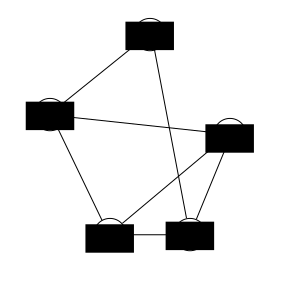
\includegraphics{img/example_graph.pdf}
  \caption{
      Visualisierung eines ungerichteten Beispielgraphs $V = \set{a, b, c, d, e},
      E = \set{(a, c), (a, e), (b, c), (b, d), (b, e), (c, d), (d, e)}$.
      Der Graph besitzt 7 von maximal 10 ($= \frac{|V| \cdot (|V|-1)}{2}$)
      Kanten. Es handelt sich um einen einfachen Graphen, der 4 Zyklen besitzt
      und planar dargestellt werden kann.
  }
  \label{fig:example_graph}
 \end{center}
\end{figure}

Ein Graph ist eine Menge $(V, E)$ von Knoten (engl. vertex) und Kanten (engl. edge). Graphen unterscheiden sich aufgrund ihrer Eigenschaften in Form und Anzahl an Knoten und Kanten. Da Graphen so vielfältig eingesetzt werden, haben sich viele Begriffe etabliert, die teilweise mehrdeutig verwendet werden. Es sei hier eine möglichst genaue Definition der Begriffe im Kontext der Informatik gegeben.

\section{Terminologie}
\index{Clique}
%
\begin{description}
  \item[(un)gerichteter Graph]
    Ein gerichteter Graph unterscheidet zwischen einer Kante $(u, v)$ und der Kante $(v, u)$, während diese Unterscheidung beim ungerichteten Graphen wegfällt. Bei einer Visualisierung werden Pfeile genutzt, um die Richtung einer Kante anzugeben.
  \item[Pfad / Weg]
   Unter einem Pfad (oder Weg) versteht man eine Sequenz von Kanten, die einer Wanderung durch den Graphen entspricht (Endknoten sind Startknoten der nächsten Kante).
  \item[Zyklus]
   Ein Pfad dessen Startknoten gleich dem Endknoten ist.
  \item[Schleife]
   Eine Kante, die den Knoten mit sich selbst verbindet. Sie ist auch damit ein Zyklus der Länge 1.
  \item[Multigraph]
    Graph, welcher mehrere Kanten zwischen zwei Knoten und Schleifen erlaubt.
  \item[einfacher/simpler Graph]
    Ungerichteter Graph, welcher kein Multigraph ist.
  \item[Baum]
   Ein Baum wird als zusammenhängender, zyklusfreier Graph verstanden. Er ermöglicht es Daten einer hierarchischen Struktur abzubilden.
  \item[Brücke]
   Unter einer Brücke versteht man eine Kante deren Entfernung zum Verlust der Eigenschaft ,,zusammenhängend`` des Graphens führt.
  \item[Vollständiger Graph]
   Unter einem vollständigen Graph versteht man einen Graph, in dem jeder Knoten mit jedem Knoten direkt verbunden ist.
  \item[Untergraph]
   Ein Graph $G'$, welcher eine Untermenge der Knoten von $G$ verwendet und nur jene Kanten verwendet, deren zugehörige Knoten in $G'$ enthalten sind.
  \item[Clique]
   Ein vollständiger Untergraph.
  \item[Eulerkreis]
   Der Eulerkreis ist ein spezieller Zyklus, der alle Knoten des Graphen nutzt und jede Kante genau einmal verwendet.
  \item[Grad eines Knoten]
   Der Grad eines Knotens ist definiert als die Anzahl an ein- und ausgehenden Kanten.
  \item[Hamiltonpfad]
   Unter einem Hamiltonpfad versteht man einen Pfad im Graphen, der jeden Knoten genau einmal besucht.
  \item[Planarität]
   Ein Graph ist planar, wenn er ohne Überschneidungen von Kanten auf einer 2D-Fläche gezeichnet werden kann.
  \item[Quelle/Senke]
   Unter der Quelle versteht man bei einem gerichteten Graphen einen Knoten, der nur nach außen führende Kanten besitzt. Eine Senke ist ein Knoten, der nur eingehende Kanten auf diesen Knoten besitzt.
\end{description}

\section{Datenstrukturen zur Speicherung von Graphen}
%
Für die Speicherung eines Graphen ist eine Datenstruktur erforderlich, die Knoten und Kanten abbildet. Die Knoten werden typischerweise durchnummeriert; deren Namen separat assoziativ gespeichert. Im Fokus stehen zwei verschiedene Konzepte um Kanten zu speichern:
%
\begin{description}
  \item[Inzidenzliste]
    Die Kanten werden als Paar von Knoten in einer Liste gespeichert.
  \item[Adjazenzmatrix]
    In einer Matrix der Größe $|V|\times |V|$ wird ein Eintrag $m_{i,j}$ mit einer 1 (oder einem Gewicht) besetzt,
    wenn eine Kante zwischen den Knoten $i$ und $j$ besteht.
\end{description}
